\chapter{Strukturaufklärung der Chl-Kataboliten mit ESI-MS} \label{sec:ChlKatabolitenESIMS}

\section{Beschreibung der Methode}

Mit dem Wissen über die ungefähren Retentionszeiten der \gls{Chl-K}en in der \gls{hplc} konnten diese in EPPIs gesammelt werden. Dabei wurde die aus der \gls{hplc} eluierte Flüssigkeit im Zeitrahmen des Peaks aufgenommen, in dem das Auftreten des jeweiligen \gls{Chl-K}en vermutet wird (ca. 0.5min.). Die erhaltene Lösung wurde in das Massenspektrometer eingespritzt und analysiert, wobei besonderes Augenmerk auf die Fragmentierung und insbesondere der Erstellung von Fragmentierungsdiagrammen gelegt wurde. 

Die Fragmentierungsdiagramme werden hier nicht diskutiert, da dies den Umfang der Arbeit deutlich sprengen würde. 

\section{Identifizierte Chl-Kataboliten}

Im Folgenden finden sich jene \gls{Chl-K}en, die über diese Methode genauer charakterisiert werden konnten (dies umfasst nicht alle mit \gls{lcms} beobachteten - siehe Tabelle \ref{tab:LCMSKatabolitenRP}). 

\subsection{Bo-DYCC}

\begin{figure}[!htbp]
  \centering
  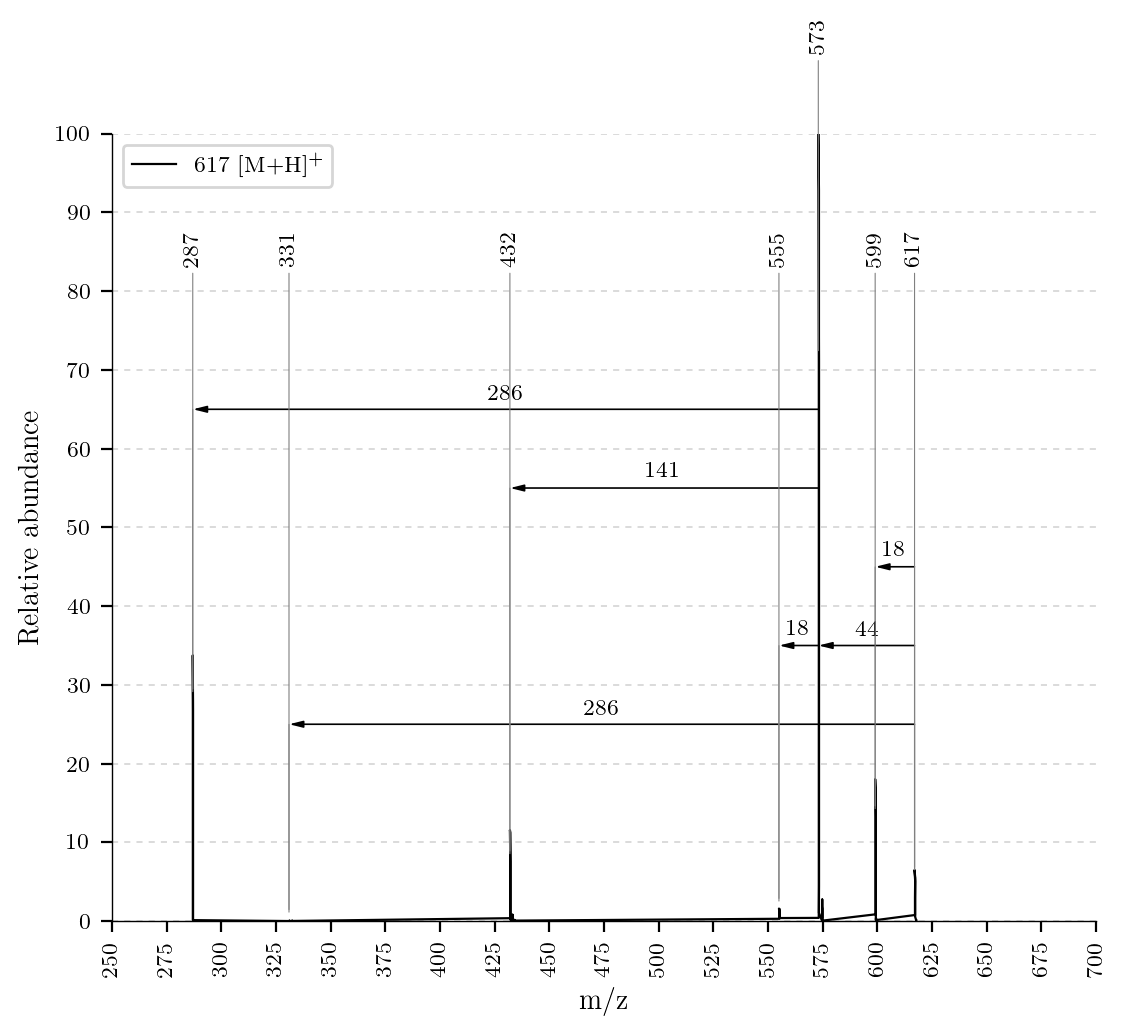
\includegraphics[width=\textwidth, height=0.6\textwidth]{figures/Kapitel7/Kataboliten/VWA_MS_617.png}
  \caption[ESI-MS Spektrum von Bo-DYCC, Quelle: Autor]{ESI-MS Spektrum von Bo-DYCC mit m/z = 617 [M+H]\textsuperscript{+}}
  \label{fig:617MH}
\end{figure}

Dieser \gls{Chl-K} konnte mit der Methode von MS Leafspray nicht gefunden werden. Mit einem hochauflösenden Massenspektrometer wurde er mit m/z = 617 [M+H]\textsuperscript{+} identifiziert. Es wurden Abspaltungen von \ch{H2O} bei m/z = 599 [M - (\ch{H2O}) + H]\textsuperscript{+}, von \ch{CO2} bei m/z = 573 [M - (\ch{CO2}) + H]\textsuperscript{+}, von Ring A bei m/z = 432 [M - (Ring A) + H]\textsuperscript{+} und von Ring C und D bei m/z = 331 [M - (Ring C, Ring D) + H]\textsuperscript{+} (Abbildung \ref{fig:617MH}) beobachtet.

Die Struktur des Bo-DYCC  wird wie in Abbildung \ref{fig:617MHStruktur} vorgeschlagen. Aufgrund der \ch{CO2} Abspaltung wird eine freie Carbonsäure an Position 8\textsuperscript{2} angenommen. Die zwei fehlenden H-Atome im Vergleich zum Bo-DNCC und die sinnvollen Zuordnungen der anderen Fragmentierungen weisen auf eine Doppelbindung an Position 16 hin.  

\begin{figure}[!htbp]
  \centering
  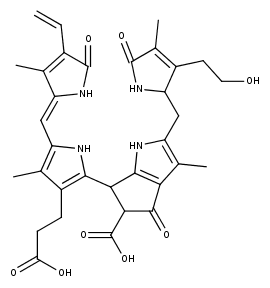
\includegraphics[scale=0.6]{figures/Kapitel7/Kataboliten/fragmentation_structures/VWA_Katabolit_617.png}
  \caption[Strukturvorschlag von Bo-DYCC, Quelle: Autor]{Strukturvorschlag von Bo-DYCC mit Summenformel \ch{C33H36N4O8}}
  \label{fig:617MHStruktur}
\end{figure}

Der Mechanismus der Abspaltung von Ring C zusammen mit Ring D wird wie in den Abbildungen \ref{fig:617MHElectronMovement} und \ref{fig:331MH} dargestellt angenommen. 

\begin{figure}[!htbp]
  \begin{subfigure}[b]{0.5\textwidth}
    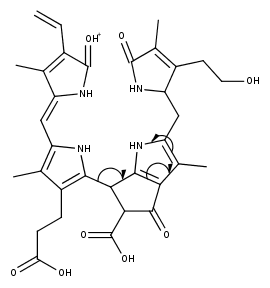
\includegraphics[width=\textwidth]{figures/Kapitel7/Kataboliten/fragmentation_structures/VWA_Katabolit_617_MH_RingD-RingC_331_electronMovement.png}
    \caption{}
    \label{fig:617MHElectronMovement}
  \end{subfigure}
  \hfill
  \begin{subfigure}[b]{0.5\textwidth}
    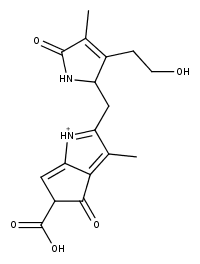
\includegraphics[width=\textwidth]{figures/Kapitel7/Kataboliten/fragmentation_structures/VWA_Katabolit_617-RingD-RingC_331.png}
    \caption{}
    \label{fig:331MH}
  \end{subfigure}
  \caption[Abspaltungsmechanismus von Ring C und Ring D bei Bo-DYCC, Quelle: Autor]{mechanistischer Vorschlag für die Abspaltung von Ring C und Ring D: (a) vorgeschlagene Bewegung der Elektronen, (b) Resultat der Abspaltung bei m/z = 331 [M - (Ring C, Ring D) + H]\textsuperscript{+} und Summenformel \ch{C17H19O5N2}}
\end{figure}

\pagebreak
\subsection{Bo-DNCC} \label{sec:ESIMSBoDNCC}

Vom Bo-DNCC wurde die protonierte Verbindung bei m/z = 619 [M+H]\textsuperscript{+} aufgenommen. Sie zeigt Abspaltungen von \ch{H2O} bei m/z = 601 [M - (\ch{H2O}) + H]\textsuperscript{+}, von \ch{CO2} bei m/z = 575 [M - (\ch{CO2}) + H]\textsuperscript{+}, von Ring D bei m/z = 452 [M - (Ring D) + H]\textsuperscript{+} und eine gemeinsame Abspaltung von Ring D und Ring A bei m/z = 311 [M - (Ring D, Ring A) + H]\textsuperscript{+} (Abbildung \ref{fig:619MH}). 

\begin{figure}[!htbp]
  \centering
  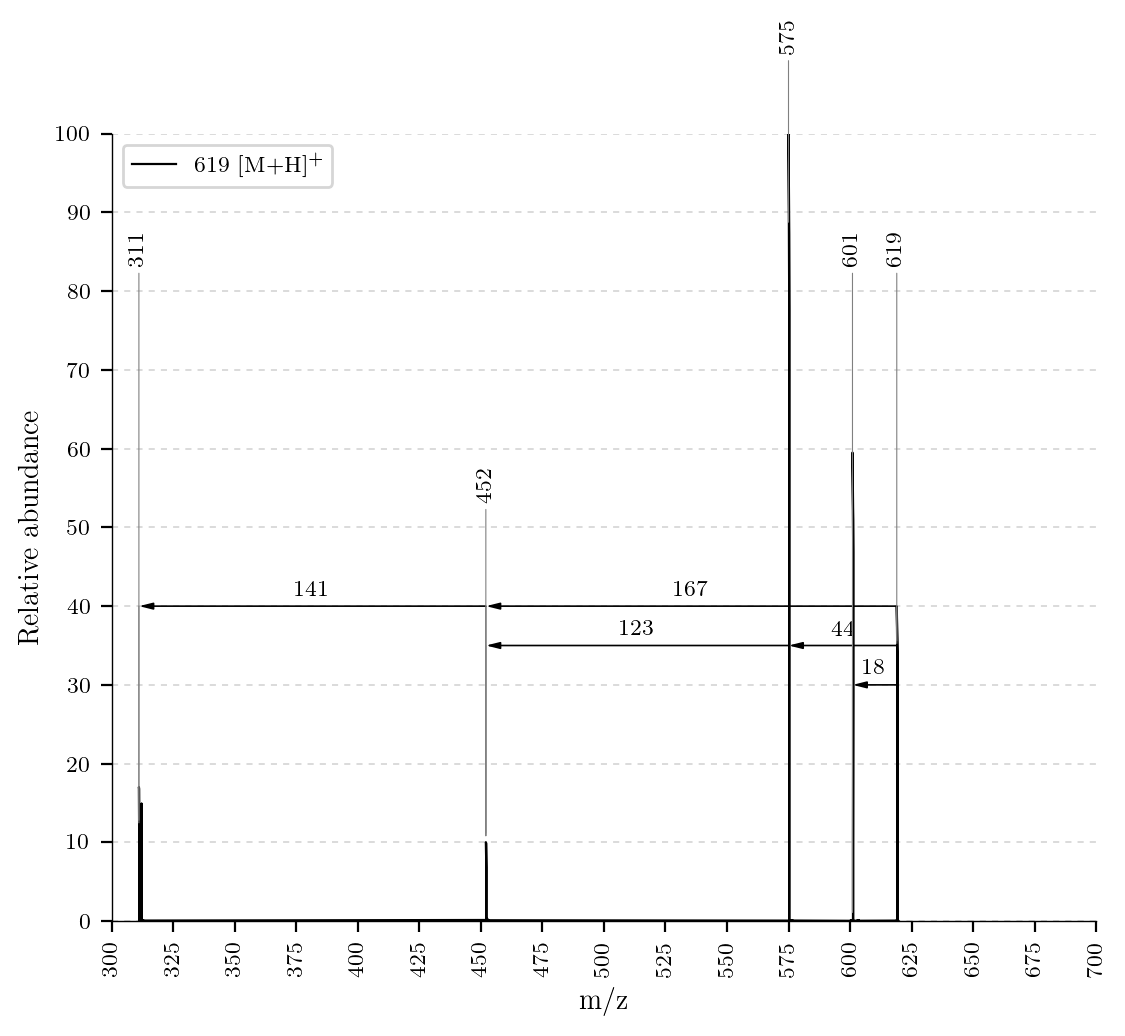
\includegraphics[width=\textwidth, height=0.7\textwidth]{figures/Kapitel7/Kataboliten/VWA_MS_619.png}
  \caption[ESI-MS Spektrum von Bo-DNCC, Quelle: Autor]{ESI-MS Spektrum von Bo-DNCC bei m/z = 619 [M+H]\textsuperscript{+}}
  \label{fig:619MH}
\end{figure}

Da für die Abspaltung von Ring A und Ring D jeweils ein Mechanismus in \cite{StructureElucidation} vorgeschlagen wird, gibt es unterschiedliche Möglichkeiten für das Abspaltungsprodukt, wenn, wie hier beobachtet, beide Ringe gleichzeitig abgespalten werden (Abbildung \ref{fig:619MHElectronMovement}). In den Abbildungen \ref{fig:311MHMesomer1}, \ref{fig:311MHMesomer2}-b werden die einzelnen Mesomere vorgeschlagen, die sich aus den Betrachtungen ergeben. 

Als stabiler werden die Mesomere bei \ref{fig:311MHMesomer2}-b aufgrund eines stabilen konjugierten Systems erachtet.

\begin{figure}[!htbp]
  \begin{subfigure}[b]{0.5\textwidth}
    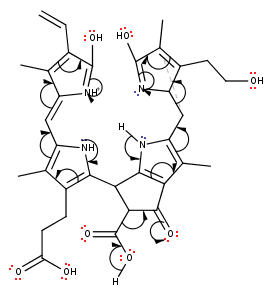
\includegraphics[width=\textwidth]{figures/Kapitel7/Kataboliten/fragmentation_structures/VWA_Katabolit_619_MH-CO2-RingA-RIngD_311_electronMovement.png}
    \caption{}
    \label{fig:619MHElectronMovement}
  \end{subfigure}
  \hfill
  \begin{subfigure}[b]{0.5\textwidth}
    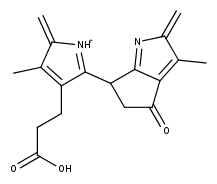
\includegraphics[width=\textwidth]{figures/Kapitel7/Kataboliten/fragmentation_structures/VWA_Katabolit_619-CO2-RingA-RingD_311.png}
    \caption{}
    \label{fig:311MHMesomer1}
  \end{subfigure}
  \caption[Abspaltungsmechanismus von Ring D und Ring A und Mesomer 1, Quelle: Autor]{vorgeschlagener Abspaltungsmechanismus von Ring D und Ring A: (a) vorgeschlagene Elektronenbewegung, (b) Mesomer 1 der Abspaltung mit m/z = 311 [M - (Ring D, Ring A) + H]\textsuperscript{+} und Summenformel \ch{C18H19O3N2}}
\end{figure}

\begin{figure}[!htbp]
  \begin{subfigure}[b]{0.5\textwidth}
    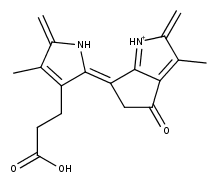
\includegraphics[width=\textwidth]{figures/Kapitel7/Kataboliten/fragmentation_structures/VWA_Katabolit_619-CO2-RingD-RingA_311_Mesomer1.png}
    \caption{}
    \label{fig:311MHMesomer2}
  \end{subfigure}
  \hfill
  \begin{subfigure}[b]{0.5\textwidth}
    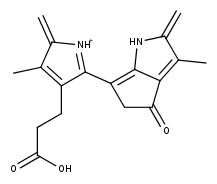
\includegraphics[width=\textwidth]{figures/Kapitel7/Kataboliten/fragmentation_structures/VWA_Katabolit_619-CO2-RingD-RingA_311_Mesomer2.png}
    \caption{}
    \label{fig:311MHMesomer3}
  \end{subfigure}
  \caption[2 Mesomere für potentielle Abspaltungsprodukte von Bo-DNCC, Quelle: Autor]{Mesomere des Abspaltungsproduktes: (a) Mesomer 2, (b) Mesomer 3}
\end{figure}

\pagebreak
\subsection{Bo-YCC}

Der Bo-YCC konnte, so wie der Bo-DYCC nicht mit MS Leafspray aufgenommen werden, dafür jedoch im Rahmen der hier verwendeten Methode. Er wurde mit m/z = 645 [M+H]\textsuperscript{+} identifiziert und zeigt Abspaltungen von \ch{H2O} bei m/z = 627 [M - (\ch{H2O}) + H]\textsuperscript{+} und von \ch{CO2} bei m/z = 601 [M - (\ch{CO2}) + H]\textsuperscript{+} (Abbildung \ref{fig:645MH}). 

\begin{figure}[!htbp]
  \centering
  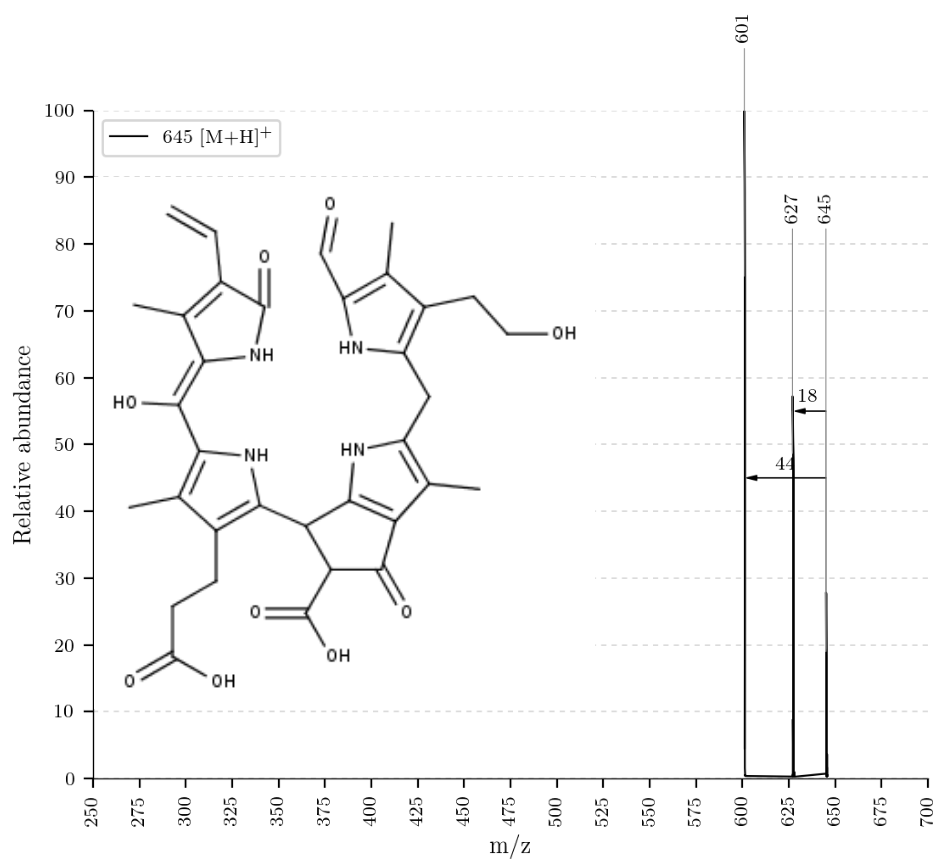
\includegraphics[width=\textwidth, height=0.8\textwidth]{figures/Kapitel7/Kataboliten/VWA_MS_645-12.png}
  \caption[ESI-MS Spektrum von Bo-YCC, Quelle: Autor]{ESI-MS Spektrum von Bo-YCC mit m/z = 645 [M+H]\textsuperscript{+} und Strukturvorschlag mit Summenformel \ch{C34H36O9N4}}
  \label{fig:645MH}
\end{figure}

Die Abspaltung von \ch{CO2} hilft, ihn vom Dimethylierungsprodukt des Bo-DYCC zu unterscheiden. Es wird deswegen an Position 8\textsuperscript{2} eine freie Carbonsäure und an Position 16 eine Doppelbindung mit einer Hydroxygruppe angenommen (Abbildung \ref{fig:645MH}).



\pagebreak
\subsection{Bo-NCC-3} \label{sec:ESIMSBoNCC3}

Der Bo-NCC-3 wurde ebenfalls wie mit MS Leafspray gefunden. Die Masse des \gls{Chl-K}en konnte bei m/z = 647 [M+H]\textsuperscript{+} bestimmt werden. Abspaltungen von \ch{H2O} bei m/z = 629 [M - (\ch{H2O}) + H]\textsuperscript{+} , von \ch{CO2} bei m/z = 603 [M - (\ch{CO2} + H]\textsuperscript{+} und von Ring D mit \ch{CO2} bei m/z = 480 [M - (Ring D-\ch{CO2}) + H]\textsuperscript{+} wurden beobachtet. 

Aufgrund der vorgeschlagenen Hydroxygruppe an Position 16 wird angenommen, dass das Abspaltungsprodukt in einem Keto-/Enolgleichgewicht steht, wie in Abbildung \ref{fig:480Mechanismus} vorgeschlagen. Mithilfe von Fragmentierungsdiagrammen könnte man argumentieren, dass diese mögliche Tautomerie aufgrund ihrer Stabilität als Triebkraft für die Abspaltung gesehen werden kann.

\begin{figure}[!htbp]
  \centering
  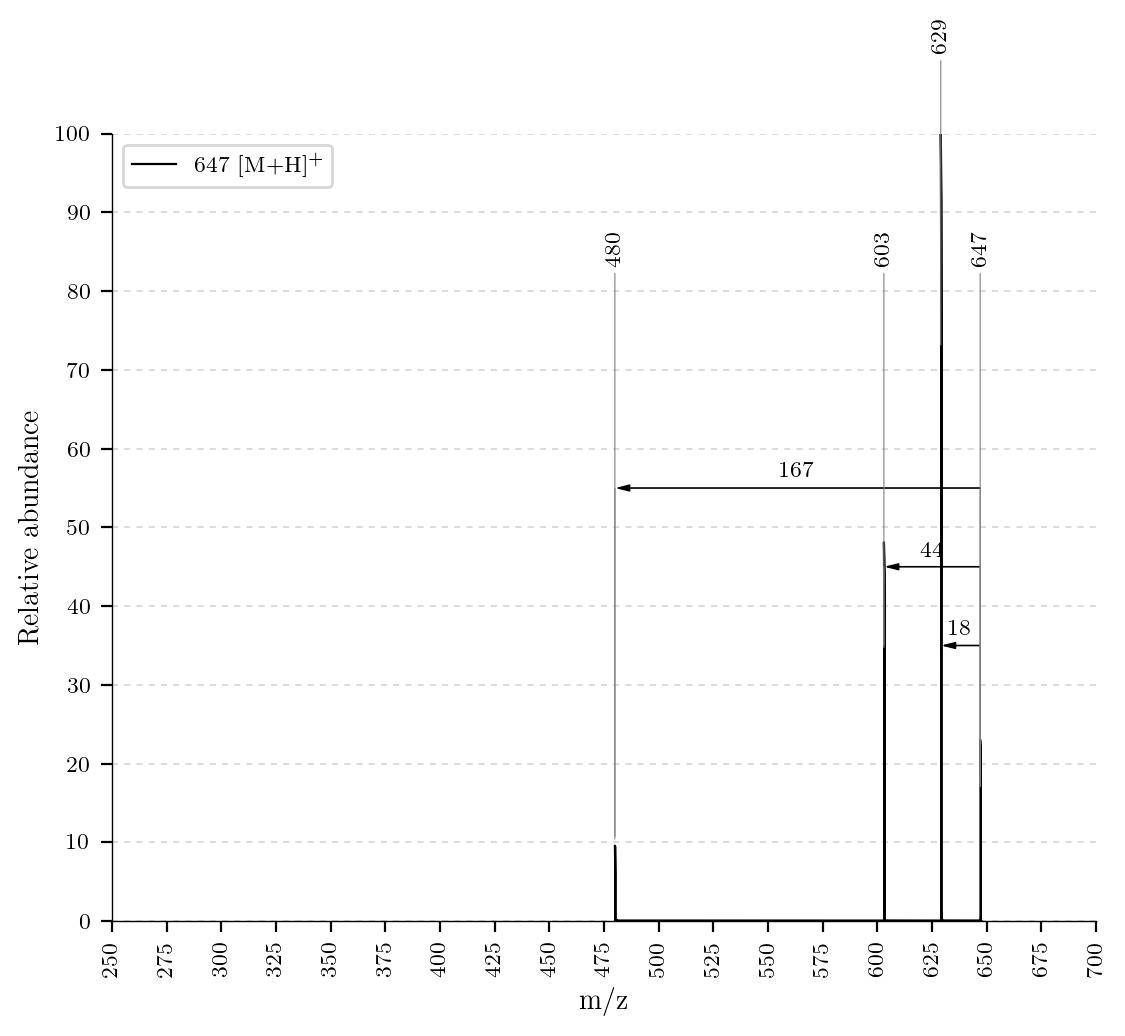
\includegraphics[width=\textwidth, height=0.6\textwidth]{figures/Kapitel7/Kataboliten/VWA_MS_647.png}
  \caption[ESI-MS Spektrum von Bo-NCC-3, Quelle: Autor]{ESI-MS Spektrum von Bo-NCC-3 mit m/z = 647 [M+H]\textsuperscript{+}}
  \label{fig:647MH}
\end{figure}

\begin{figure}[!htbp]
  \begin{subfigure}[b]{0.5\textwidth}
    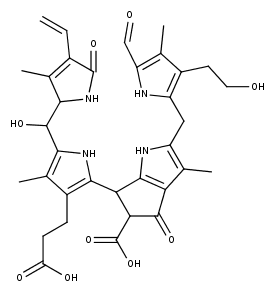
\includegraphics[width=\textwidth]{figures/Kapitel7/Kataboliten/fragmentation_structures/VWA_Katabolit_647.png}
    \caption{}
    \label{fig:647MStruktur}
  \end{subfigure}
  \hfill
  \begin{subfigure}[b]{0.5\textwidth}
    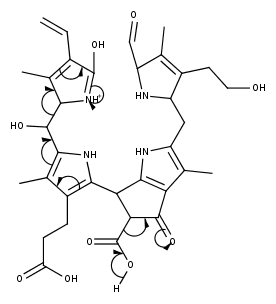
\includegraphics[width=\textwidth]{figures/Kapitel7/Kataboliten/fragmentation_structures/VWA_Katabolit_647-CO2-RingD_480_MH_electronMovement.png}
    \caption{}
    \label{fig:480Mechanismus}
  \end{subfigure}
  \caption[Strukturvorschlag von Bo-NCC-3 und Vorschlag für Mechanismus der Abspaltung von Ring D, Quelle: Autor]{(a) Strukturvorschlag von Bo-NCC-3 mit Summenformel \ch{C34H39O9N4}, (b) vorgeschlagener Mechanismus für die Abspaltung von Ring D mit \ch{CO2}}
\end{figure}

\begin{figure}[!htbp]
  \begin{subfigure}[b]{0.5\textwidth}
    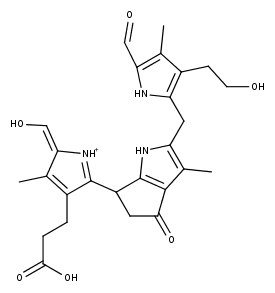
\includegraphics[width=\textwidth]{figures/Kapitel7/Kataboliten/fragmentation_structures/VWA_Katabolit_647-CO2-RingD_480_MH_Enolform.png}
    \caption{}
    \label{fig:NCC2725}
  \end{subfigure}
  \hfill
  \begin{subfigure}[b]{0.5\textwidth}
    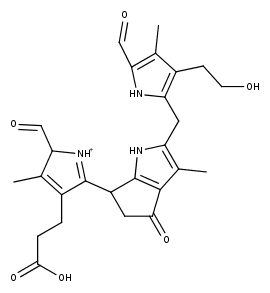
\includegraphics[width=\textwidth]{figures/Kapitel7/Kataboliten/fragmentation_structures/VWA_Katabolit_647-CO2-RingD_480_MH_Ketoform.png}
    \caption{}
    \label{fig:DNCC2991}
  \end{subfigure}
  \caption[vorgeschlagene Keto-/Enoltautomerie der Ring D Abspaltung von Bo-NCC-3, Quelle: Autor]{vorgeschlagene Keto-/Enoltautomerie beim Abspaltungsprodukt von Ring D mit Summenformel \ch{C26H30O6N3}: (a) Enolform, (b) Aldehyd (vermutlich stabiler)}
\end{figure}

\pagebreak
\subsection{Bo-NCC-1} \label{sec:ESIMSBoNCC1}

Der Bo-NCC-1 konnte bei m/z = 793 [M+H]\textsuperscript{+} aufgenommen werden. Er zeigte im Vergleich zu MS Leafspray mehr Abspaltungen, nämlich von \ch{H2O} bei m/z = 775 [M - (\ch{H2O}) + H]\textsuperscript{+} , von \ch{CO2} bei m/z = 749 [M - (\ch{CO2}) + H]\textsuperscript{+}, von Zucker bei m/z = 631 [M - (Zucker) + H]\textsuperscript{+}, von Zucker zusammen mit \ch{H2O} bei m/z = 613 [M - (\ch{H2O}) + H]\textsuperscript{+} und von Zucker zusammen mit \ch{CO2} bei m/z = 587 [M - (\ch{CO2}) + H]\textsuperscript{+}. 

Die Struktur wird wie in Abbildung \ref{fig:831MKLeafspraystructure} vorgeschlagen.

\begin{figure}[!htbp]
  \centering
  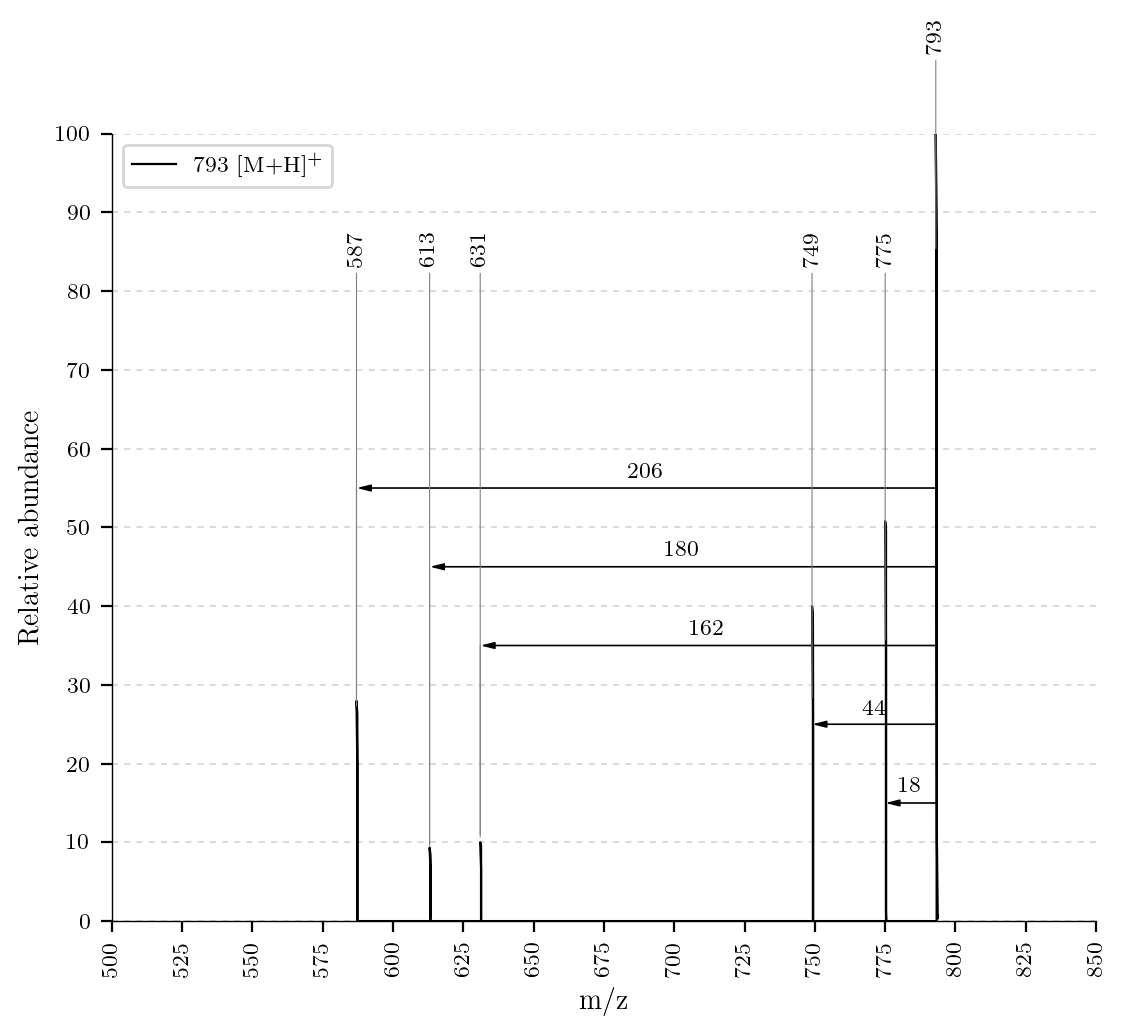
\includegraphics[width=\textwidth, height=0.7\textwidth]{figures/Kapitel7/Kataboliten/VWA_MS_793.png}
  \caption[ESI-MS Spektrum von Bo-NCC-1, Quelle: Autor]{ESI-MS Spektrum von Bo-NCC-1 mit m/z = 793 [M+H]\textsuperscript{+}}
  \label{fig:793MH}
\end{figure}



\pagebreak
\section{Reaktionsprodukte der Chl-Kataboliten}

\subsection{Reaktionsprodukte von Bo-DYCC}

Vom Bo-DYCC konnten zwei Reaktionsprodukte gefunden werden, eines bei m/z = 631 [M+H]\textsuperscript{+} und eines bei m/z = 645 [M+H]\textsuperscript{+}. Beim ersten handelt es sich um einen Methylester. Dieser wird an Position 12\textsuperscript{3} vermutet, da das Ion eine Abspaltung von \ch{CO2} bei m/z = 587 [M - (\ch{CO2}) + H]\textsuperscript{+} zeigt (Abbildung \ref{fig:631MH}). 

Beim Reaktionsprodukt bei m/z = 645 [M+H]\textsuperscript{+} handelt es sich um einen Dimethylester, an den Positionen 8\textsuperscript{2} und 12\textsuperscript{3}.  Dies zeigt die Abspaltung von \gls{meoh} bei m/z = 613 [M - (\gls{meoh}) + H]\textsuperscript{+} (Abbildung \ref{fig:645MH}). 

Dies ist überraschend, da bei den meisten anderen untersuchten \gls{Chl-K}en die Bildung eines Monomethylesters an Position 8\textsuperscript{2} beobachtet wurde, welche durch das häufige natürliche Vorhandensein von Methylestern als günstiger angesehen werden kann.

\begin{figure}[!htbp]
  \centering
  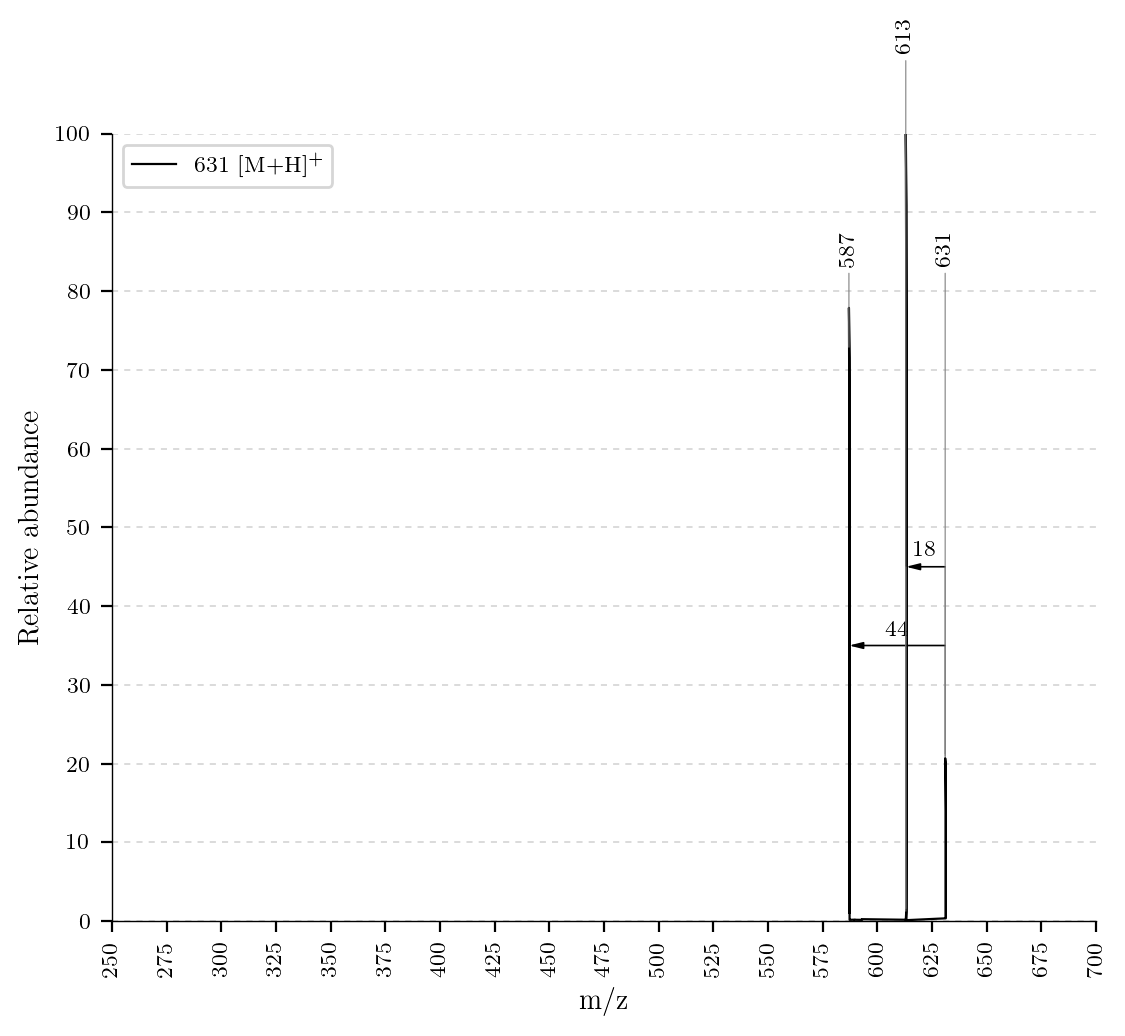
\includegraphics[width=\textwidth, height=0.7\textwidth]{figures/Kapitel7/Kataboliten/VWA_MS_631.png}
  \caption[ESI-MS Spektrum des Monomethylesters von Bo-DYCC, Quelle: Author]{ESI-MS Spektrum des Monomethylesters von Bo-DYCC bei m/z = 631 [M+H]\textsuperscript{+}}
  \label{fig:631MH}
\end{figure}

\begin{figure}[!htbp]
  \centering
  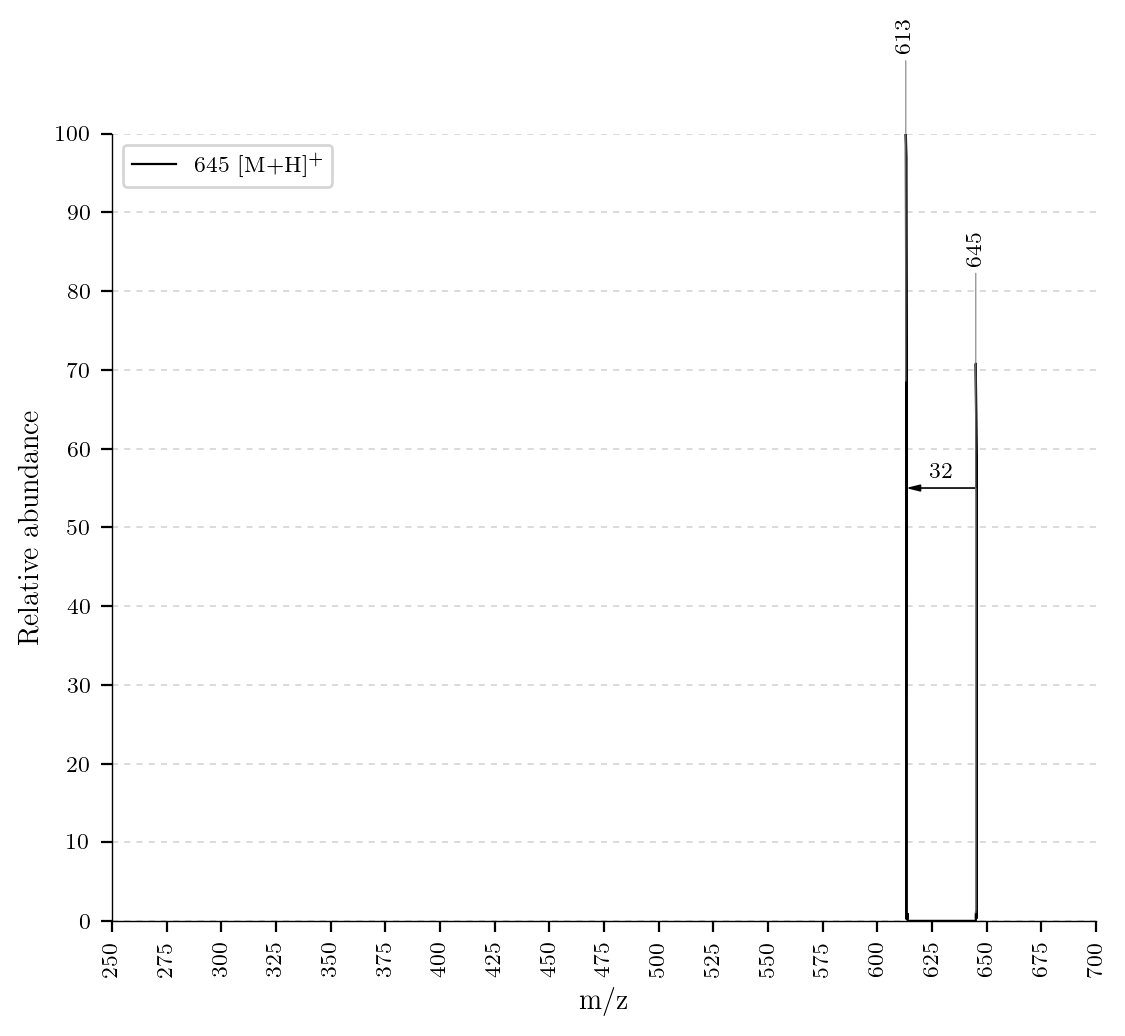
\includegraphics[width=\textwidth, height=0.6\textwidth]{figures/Kapitel7/Kataboliten/VWA_MS_645-2.png}
  \caption[ESI-MS Spektrum des Diethylesters von Bo-DYCC, Quelle: Author]{ESI-MS Spektrum des Dimethylesters von Bo-DYCC bei m/z = 645 [M+H]\textsuperscript{+}}
  \label{fig:645MH}
\end{figure}


\begin{figure}[!htbp]
  \begin{subfigure}[b]{0.5\textwidth}
    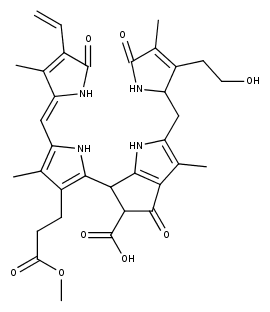
\includegraphics[width=\textwidth]{figures/Kapitel7/Kataboliten/fragmentation_structures/VWA_Katabolit_631.png}
    \caption{}
    \label{fig:631MHStruktur}
  \end{subfigure}
  \hfill
  \begin{subfigure}[b]{0.5\textwidth}
    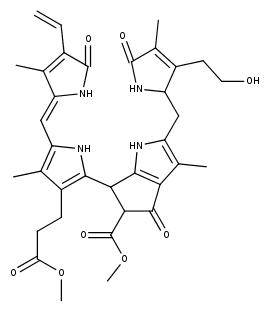
\includegraphics[width=\textwidth]{figures/Kapitel7/Kataboliten/fragmentation_structures/VWA_Katabolit_645_nachReaktion.png}
    \caption{}
    \label{fig:645MHStruktur}
  \end{subfigure}
  \caption[Strukturvorschläge für das Mono- und Dimethylierungsprodukt des Bo-DYCC, Quelle: Autor]{Strukturvorschläge: (a) Monomethylierungsprodukt mit Summenformel \ch{C34H38O8N4}, (b) Dimethlyierungsprodukt mit Summenformel \ch{C35H41O8N4}}
\end{figure}

\subsection{Reaktionsprodukt von Bo-DNCC}

Das Reaktionsprodukt des Bo-DNCC wurde bei m/z = 633 [M+H]\textsuperscript{+} gefunden. Aufgrund der Abspaltung von \ch{meoh} wird angenommen, dass sich der Methylester an Position 8\textsuperscript{2} ausbildet. Auf eine Diskussion aller in Abbildung \ref{fig:633MH} ersichtlichen Fragmentierungen wird ob der Menge verzichtet.

\begin{figure}[!htbp]
  \centering
  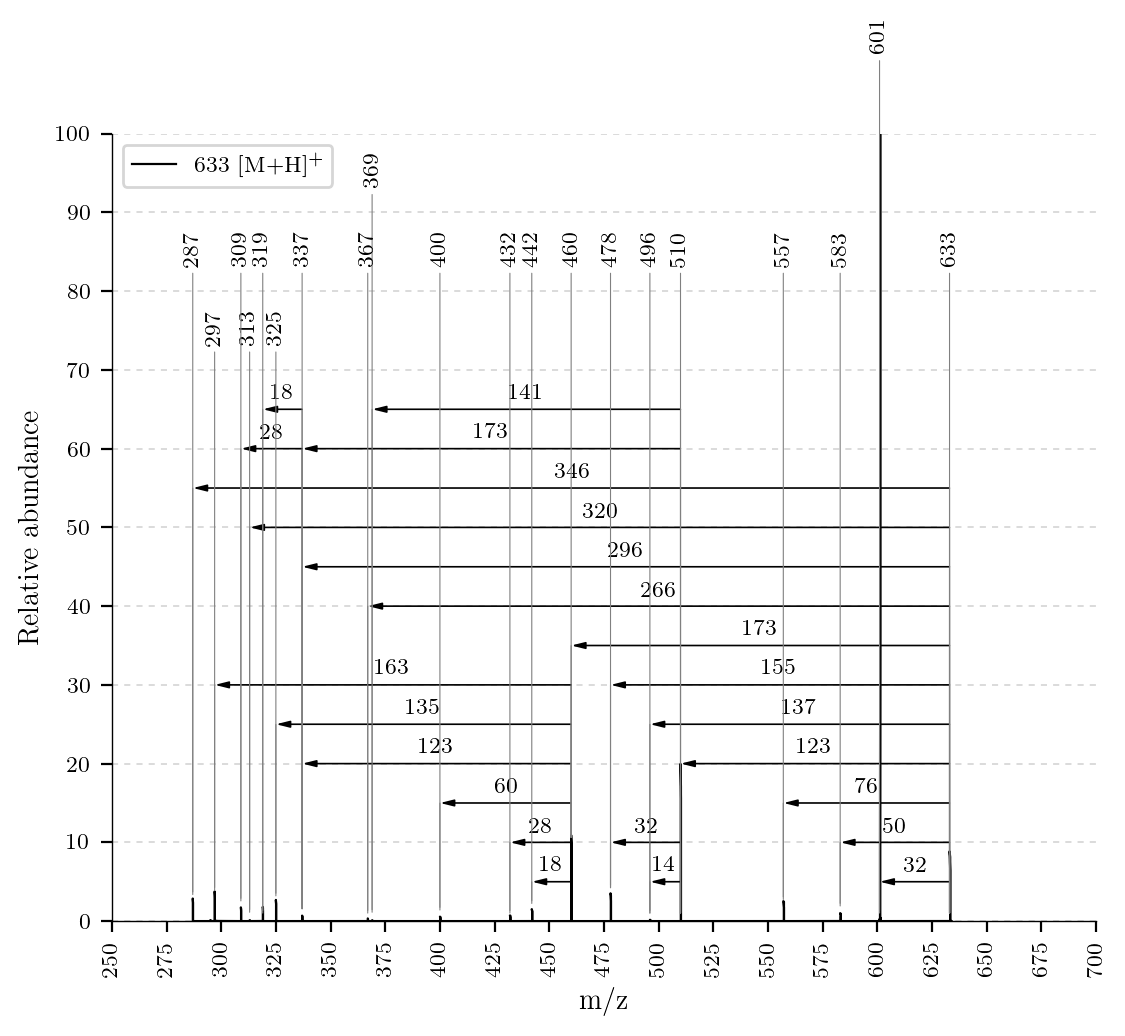
\includegraphics[width=\textwidth, height=0.7\textwidth]{figures/Kapitel7/Kataboliten/VWA_MS_633.png}
  \caption[ESI-MS Spektrum des Reaktionsproduktes von Bo-DNCC, Quelle: Autor]{ESI-MS Spektrum des Reaktionsproduktes des Bo-DNCC mit m/z = 633 [M+H]\textsuperscript{+}}
  \label{fig:633MH}
\end{figure}

\begin{figure}[!htbp]
  \centering
  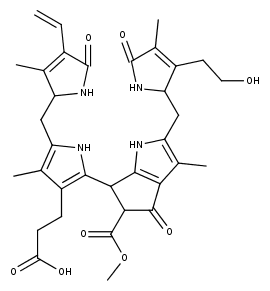
\includegraphics[scale=0.6]{figures/Kapitel7/Kataboliten/fragmentation_structures/VWA_Katabolit_633.png}
  \caption[Strukturvorschlag für das Reaktionsprodukt von Bo-DNCC, Quelle: Autor]{Strukturvorschlag für das Reaktionsprodukt von Bo-DNCC mit Summenformel \ch{C34H41O8N4}}
  \label{fig:633MStruktur}
\end{figure}

\pagebreak
\subsection{Reaktionsprodukt von Bo-YCC}

Das Reaktionsprodukt des Bo-DYCC konnte nicht gesammelt werden, weswegen keine weiteren strukturellen Informationen vorhanden sind. Es wurde lediglich im \gls{lcms} Lauf identifiziert (Tabelle \ref{tab:LCMSKatabolitenRP}).

\subsection{Reaktionsprodukt von Bo-NCC-1}

Das Reaktionsprodukt des Bo-NCC-1 konnte ebenfalls nicht gesammelt und näher identifiziert werden. Es wurde aber im \gls{lcms} identifiziert (Tabelle \ref{tab:LCMSKatabolitenRP}).

\pagebreak
\subsection{Reaktionsprodukt von Bo-NCC-3} \label{sec:ESIMSRPBoNCC3}

Das Reaktionsprodukt des Bo-NCC-3 konnte bei m/z = 661 [M+H]\textsuperscript{+} identifiziert werden und zeigte, so wie das Reaktionsprodukt von Bo-DNCC eine große Anzahl an Fragmentierungen (Abbildung \ref{fig:661MH}). 

\begin{figure}[!htbp]
  \centering
  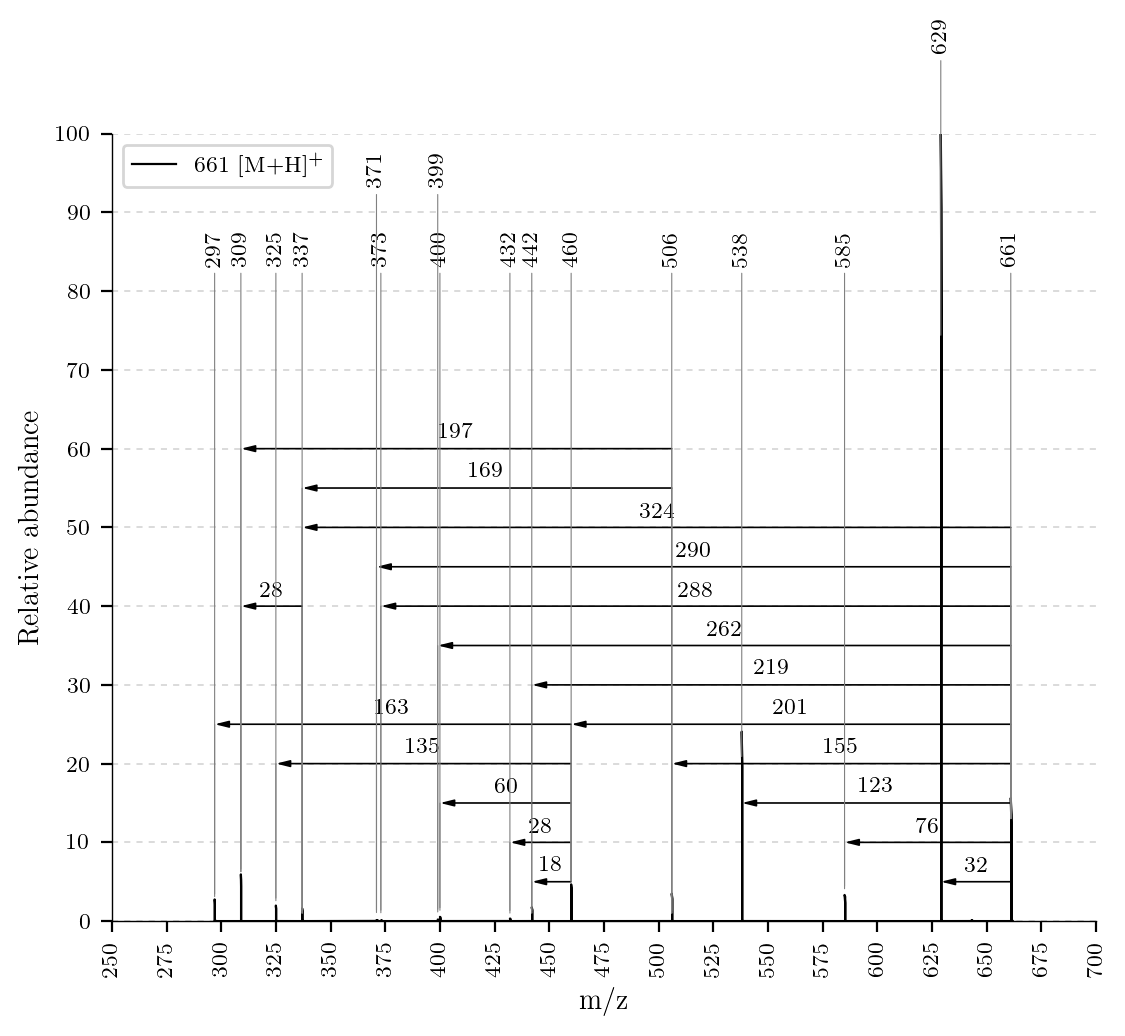
\includegraphics[width=\textwidth, height=0.7\textwidth]{figures/Kapitel7/Kataboliten/VWA_MS_661.png}
  \caption[ESI-MS des Reaktionsproduktes von Bo-NCC-3, Quelle: Author]{ESI-MS des Reaktionsproduktes von Bo-NCC-3 bei m/z = 661 [M+H]\textsuperscript{+}}
  \label{fig:661MH}
\end{figure}

